\documentclass[12pt]{article}

\title{Creating A Student Scheduling Database}
\date{December 6th, 2024}

% author hijacking is so real https://tex.stackexchange.com/questions/63384/add-additional-text-on-title-page
\author{\parbox{\linewidth}{\centering%
	Team Debian
	\endgraf\bigskip
	Jerry Cai, Paa Kweku Cato, Drew Fischer, Akhmad Mamirov, Will Sieber
	\bigskip
}}

\usepackage[left=1in,right=1in,top=1in,bottom=1in]{geometry}
\usepackage{graphicx} %package to manage images
\usepackage{setspace}

\spacing{1.5}

\begin{document}
\maketitle

% Latex can automatically build a table of contents for you
\newpage
\tableofcontents
\newpage

\section{Abstract}
This semester, our group developed an enhanced course scheduling system for students in our Database Systems class. We analyzed the Self Service platform’s user interface to understand current data organization and management, as we lacked direct access to the underlying records. We gathered user feedback through student interviews, using both open-ended and close-ended questions to identify their experiences and suggestions for improvement. Based on this analysis, we designed a new database structure with a preliminary list of fields and table specifications, ensuring data integrity and consistency through a business rule specification sheet and validation tables. We created view specifications for easy data access and reporting, and an Entity-Relationship Diagram (ERD) to illustrate the database schema and relationships. Our final design includes tables for students, courses, instructors, prerequisites, enrollments, classrooms, and schedules, all aimed at providing greater insight and flexibility for course selection. Additionally, we developed a user-friendly interface using HTML and CSS, creating a clean and intuitive layout for the scheduling system. Our Golang backend efficiently handles data operations and ensures seamless communication between the UI and database, offering scalability and security. Together, the HTML/CSS UI and Golang backend provide a cohesive and reliable system, enhancing the overall user experience and better meeting student needs.

\newpage

\section{Introduction}

\subsection{Background}
In the modern academic world, students often are faced with challenges when it comes to scheduling their courses. Conflicts in timing, prerequisite requirements, and instructor availability prove to be difficult for students to create a schedule that balances their academic needs and personal preferences. Recognizing these challenges, our team set out to develop a comprehensive scheduling system with our primary objective being to create a user-friendly scheduling system that helps students optimize their course selections based on several factors including course prerequisites, instructor availability, and classroom capacity. By offering a centralized platform for managing course enrollments and schedules, we aim to enhance students' academic success and overall learning experience.

\subsection{Motivation}
There were a few reasons we chose to focus on student scheduling and grade information for our database’s contents. Firstly, there was an inherent familiarity with the concepts involved; all of us are very experienced with scheduling classes and looking at grades through Wooster’s Colleague Self Service portal. We predicted that this existing familiarity would be a significant help in identifying the subjects and characteristics we would need to implement in the database.

Secondly, we had a robust and well-designed existing database to take inspiration from. The aforementioned Self Service portal has most of the information we would conceivably use, and while we obviously don’t have administrative access, we can look at our own records collectively and use what we’ve learned in class to extrapolate backwards and determine what the structure would have to be to facilitate the information we can see.

\subsection{Goals}
Our main goal is to gain in-depth learning and mastery of SQL skills by creating a database for student course scheduling and to understand the ways in which database design can be applied in real-world scenarios. Through this project, we hope to not only deepen our understanding of classroom knowledge, but also explore how theoretical concepts can be effectively applied to solve real-world problems. Ultimately, our goal is to design an efficient, intuitive, and practically relevant database system that will provide a reliable support tool for students' course scheduling and academic planning.

\subsection{Database Design Overview}
The database design process began with a thorough analysis of the requirements for the student scheduling system. We identified key entities such as students, courses, enrollments, prerequisites, and instructors and defined their attributes and relationships. We then designed the database schema, ensuring normalization to reduce redundancy and improve data integrity. We carefully selected primary and foreign keys to create clear relationships between tables, while attributes were chosen to provide insight into students' course schedules and academic performance. Lastly, we created views to simplify complex queries and provide tailored views of the data for different users. Throughout the design process, we focused on scalability and usability, aiming to create a robust system that meets real-world needs.

\subsection{Application Implementation Overview}
The application implementation focused on combining the database structure with the user requirements. By separating the application into a front-end and a back-end, one can query the database server-side and send the requested information back to the user. In the front-end, a user interface was written in pure HTML/CSS to create an efficient and friendly environment to view data and add entries. To enable front-end and back-end communication, we relied on AJAX methods through which data from the database is passed to the user interface.


\section{Database Design}

\subsection{Introduction}
Database design is the core part of the entire project, determining the functionality, scalability, and efficiency of the system's data management. With the goal of supporting students' course scheduling, our design aims to create a database system that is both well-structured and flexible. During the design process, we took into account the delineation of entities and relationships, the minimization of data redundancy, and the needs of different user roles (e.g., students, lecturers, and administrators). By strictly following the principles of database normalization, we ensure data integrity and consistency, while providing a good foundation for subsequent queries and functional extensions.

\subsection{Starting the Process}
The initial focus of the project was to develop a clear mission statement and specific objectives to guide the development of the database system. Our mission was to create a reliable, user-friendly student schedule database that would meet the challenges of course management and academic planning. Broadly speaking, our goal was to simplify the process of organizing course schedules and managing academic data while ensuring scalability and adaptability to accommodate future improvements.

To accomplish this, we set specific goals, including creating a normalized table structure, implementing robust relationships between entities, and designing the user interface to seamlessly interact with the database. In addition, we used informal interviews and discussions to understand user needs and gather the experiences of peers and academic advisors with existing scheduling systems. These insights helped us identify pain points, such as difficulties in navigating course prerequisites and inefficiencies in viewing enrollment data, to orient our project goals. This early phase provided a solid foundation for the design and implementation phases of our database system.

\subsection{Analyzing the Current Database}
In our analysis of the current database, we did not have access to the actual records of the existing Self Service database. Instead, we examined how the data is presented and managed through its user interface. This approach allowed us to gather insights into the structure and functionality of the existing system.

\subsubsection*{Data Management}

To document how data is presented and managed in the current system, we conducted a detailed analysis of the Self Service platform's UI. Our findings are as follows:

\begin{itemize}
  \item  \textbf{Data Presentation}: In the Self Service platform, data can be accessed via multiple pages such as Grades, where the courses a student has taken are grouped by semester and displayed with their final grade; or Search for Courses, where students can filter the list of every course offered in the coming semester. The UI provides a clear, albeit limited, view of how the data is organized and displayed.
  \item \textbf{Data Management}: Data management in the current system involves user interactions with the UI in situations such as students register for courses or when advisors release students to do so. This process can be as the system's limited integration between different data sections makes it difficult to obtain a comprehensive view of the scheduling process.
\end{itemize}

\subsubsection*{User Interviews}

To gather user feedback and identify areas for improvement, we conducted interviews with students at The College of Wooster. The focus of these interviews was the Self-Service platform, which is used for course planning and registration. Our approach included the following methods:

\begin{itemize}
  \item  \textbf{Open-Ended Questions}:  We asked students open-ended questions to gain insights into their experiences with the current system and to understand their needs and preferences like: "Can you describe your experience with the Self-Service platform when planning your courses?". This approach allowed us to capture a wide range of feedback and identify common themes.
  \item \textbf{Closed-Ended Questions}: We also used closed-ended questions to collect specific data points about the usability and functionality of the Self-Service platform. We asked: "On a scale of 1 to 5, how easy is it to navigate the Self-Service platform?" (1 being very difficult, 5 being very easy) "Do you find the course search feature helpful? (Yes/No)". This helped us quantify the frequency of certain issues and preferences among students.
  \item \textbf{Subject Identification Technique (SIT)}: We used SIT to identify the main subjects or entities relevant to course scheduling, such as courses, students, instructors, and classrooms. This technique helped us ensure that our database design would cover all necessary aspects.
  \item \textbf{Character Identification Technique (CIT)}: CIT was employed to identify the characteristics or attributes of each subject. For example, for the course entity, we identified attributes such as course code, title, description, credits, and prerequisites.
\end{itemize}


\subsection{Establishing Table Structures}
When figuring out which table we would need, we started with the obvious: Students, Courses, and Instructors (all Data tables). From there, we created a Linking table called Enrollments that would connect Students to Courses, keeping track of which students took what courses, and when. Finally, we added a Prerequisites table to contain the prerequisites each course requires for it to be taken. By keeping the table structure as simple as possible, it was very easy to make our tables ideal. We were also able to create many ideal fields by splitting up first and last names, and by creating ID numbers for students and professors. The following ER Diagram describes each table and their characteristics:

\begin{figure}[h]
    \centering
    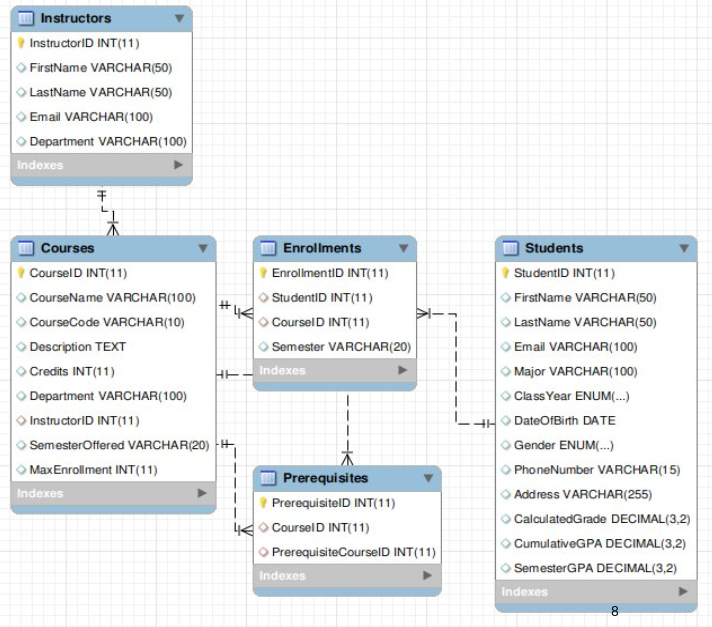
\includegraphics[width=1\textwidth]{images/img4.png}
    \caption{ER Diagram of the Database.}
    \label{fig:mesh1}
\end{figure}


\subsection{Keys}
During the database design process, we select primary and foreign keys primarily by analyzing the core attributes of each table. Due to the small number of candidate keys for each table, choosing a primary key is relatively straightforward. We make sure that the primary key of each table uniquely identifies the record, creating a StudentID for the Student table, CourseID for the Course table, and EnrollmentID for the Enrollment table. these fields are not only easy to generate, but also effective in preventing duplicate data.

The selection of foreign keys is based on the relationship between tables. In order to establish a clear association, we use the foreign keys StudentID and CourseID in the enrollment table to refer to the primary keys of the student table and the course table, respectively, to realize the one-to-many relationship between students and courses. In addition, the CourseID and PrerequisiteCourseID foreign keys in the PrerequisiteCourse table ensure the association between a course and its prerequisite requirements. The selection of these key fields not only ensures the logical integrity of the database, but also provides support for complex queries and data analysis.

\subsection{Field Specifications}
Nearly all the fields in our database are either nominal, numerical, or identity-verifying in nature. The numerical fields include numerical descriptors such as a student’s GPA or how many credits a class is worth. The nominal fields contain names, descriptions, and identifying information such as email addresses or department names; anything that needs text to describe it. The identification fields, as mentioned in the previous section, create unique identifiers for many of the nominal elements in the database.

\subsubsection*{Physical elements}

For the nominal fields, most are intended to be unique, and are length-limited to values depending on context; for example, first and last names have a limit of 50 characters while addresses – typically much longer – have a limit of 255. The physical elements of the numeric values vary, but all the GPA values will be limited to two decimal places. ID numbers are not limited at all, but since we don’t expect the number of students to exceed two billion, integers should be sufficient.

\subsubsection*{Logical Elements}

Currently, all elements are entered by users and are allowed to be null. This isn’t ideal for long-term use, and we will work in the future to modify the fields, so we don’t end up with partial and incomplete entries. Similarly, we don’t have any ranges implemented yet. Ideally, for the numeric fields would limit GPA to values between 0 and 4 and course credits to values between 0 and 2. Few nominal fields would need pre-specified ranges, but some examples are Department, Major, and CourseCode, which would need each value to be determined so users couldn’t misspell anything or make up an imaginary course.

\subsection{Table Relationships}
Due to the small number of tables and the nature of our design, all five tables have many-to-many relationships with one another. Multiple students take each single course, a single course can have multiple professors, each student makes multiple enrollments each semester, and a course can have multiple prerequisites. In the future, we hope to add deletion rules to account for students dropping out and degree of participation limits to make sure students aren’t signing up for more courses than they’re allowed to take.

\subsection{Business Rules}
In database design, business rules are an important part of ensuring data integrity and operational standardization. We have formulated a series of business rules based on project requirements, which can be divided into two categories: database-oriented rules and application-oriented rules.

Database-oriented rules are mainly realized at the database level through Constraints and Triggers. For example, in the Student table, we use field constraints to ensure that each student's Email is unique and to limit the grade field to a valid range (e.g., 0 to 4.0). In addition, in the Enrollment table, foreign key constraints are used to ensure that each enrollment record is associated with a valid student and course. These rules directly maintain data integrity and consistency through internal database mechanisms.

Application-oriented rules, on the other hand, rely more on front-end or back-end logical processing. For example, during the course registration process, the system checks to see if a student has completed the required prerequisite courses. Although these rules are based on data in the database, the implementation logic is located in the application code rather than in the database itself. In terms of rule specifics, our business rules include both field-specific rules (e.g., grade ranges and uniqueness) and relationship-specific rules (e.g., one-to-many relationships between students and courses).

\subsection{Views}
In the project, we designed a series of Views to simplify complex query operations, improve data access efficiency, and provide customized data presentation for different user needs. These views can be categorized into three main types: Data Views, Aggregate Views and Validation Views.

The primary function of a Data View is to provide a clear set of data extracted from the underlying table. For example, we created a view to display information about each student's enrolled courses and corresponding credits. This view integrates data from the Student, Enrollment, and Course tables, simplifying the process of querying student course information while avoiding the complexity of directly manipulating the base table.

Aggregate views are used to generate results based on statistics and summaries. A typical aggregated view is one that displays the number of students enrolled in each course along with instructor information. This view provides intuitive statistical support for course management by aggregating data from the enrollment table, calculating total enrollment for each course, and combining it with information from the instructor table.

The role of validation views is to assist in checking and ensuring the integrity of data. For example, a view was designed to display all enrollment records that do not meet prerequisite course requirements. This view helps administrators to quickly identify potential data issues and take appropriate action to correct them, thus improving the accuracy and reliability of the system.

\subsection{Data Integrity}

As previously stated, our mission was to design a database that improves the course scheduling system by providing students with greater insight and flexibility in course selection. We met this objective by creating a structured database that ensures data accuracy and consistency across all entities—students, courses, instructors, prerequisites, and enrollments. We reviewed each table and its fields to ensure that they are ideal for maintaining data integrity:

\begin{itemize}
  \item \textbf{Students Table}: Captures essential student information such as student id, firstname, lastname .etc. This ensures accurate identification and record-keeping.

  \item \textbf{Courses Table}: Contains course details such as course code, course name, and credits, ensuring clear organization and minimizing errors.

  \item \textbf{Instructors Table}: Links instructors to courses, ensuring accurate instructor assignment to courses.

  \item \textbf{Prerequisites Table}: Tracks course prerequisites to ensure students meet necessary requirements before enrolling.

  \item \textbf{Enrollments Table}: Tracks student enrollments, semesters, and course id, ensuring accurate academic records.
\end{itemize}

Our relationships are entirely many-to-many, ensuring proper linkage between related data while preventing duplication. We validated the fields and ensured that each table’s structure supports efficient and consistent data management. This design maintains data integrity and supports the goals of the course scheduling system.

\newpage

\section{Application Implementation}
\subsection{Introduction}
Creating an application involves three distinct components – a front-end user interface, a back-end webserver, and the communication between the two. The front-end allows managers and users to view the database. The back-end webserver allows one to query the MySQL database. By allowing communication between the front-end and the back-end, one can deploy a website that allows managers to keep track of students, classes, and professors.

\subsection{Software and Tools Used}
To create a webserver, the Golang programming language was used. Golang’s \textit{net/http} library was used to handle http requests made by a user, and the \textit{database/sql} library was used to query the database with SQL commands when desired. Communication between the front-end and back-end was done via Javascript, with the help of jQuery. jQuery's \textit{\$.ajax} function sends a GET request to the server, which signals the back-end to execute a SQL query. A .json file is sent back in return, which is parsed into several HTML tags that are displayed on the webpage.

\subsection{Application Demonstration}
The navbar provides three separate pages that users can view: a “welcome” page, a “view database” page, and a “add entry” page. The “welcome” page introduces users to the website and provides links to several pages that one can view.

\begin{figure}[h]
    \centering
    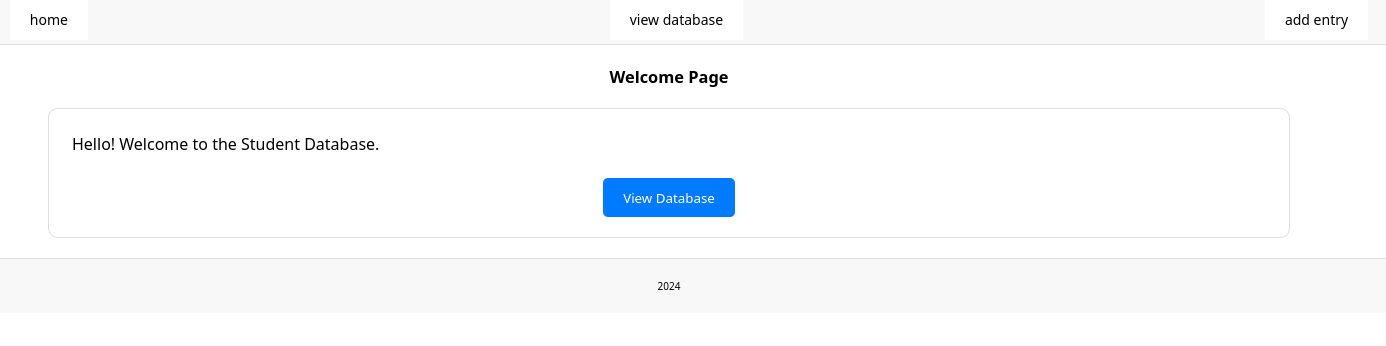
\includegraphics[width=1\textwidth]{images/img1.png}
    \caption{The Welcome page.}
    \label{fig:mesh1}
\end{figure}

The “view database” page communicates with the back-end upon page load, which is described in the previous section. The “add entry” page allows users to enter new students from the front-end, which likewise executes a SQL query similar to that of the “view databases” page.

\begin{figure}[h]
    \centering
    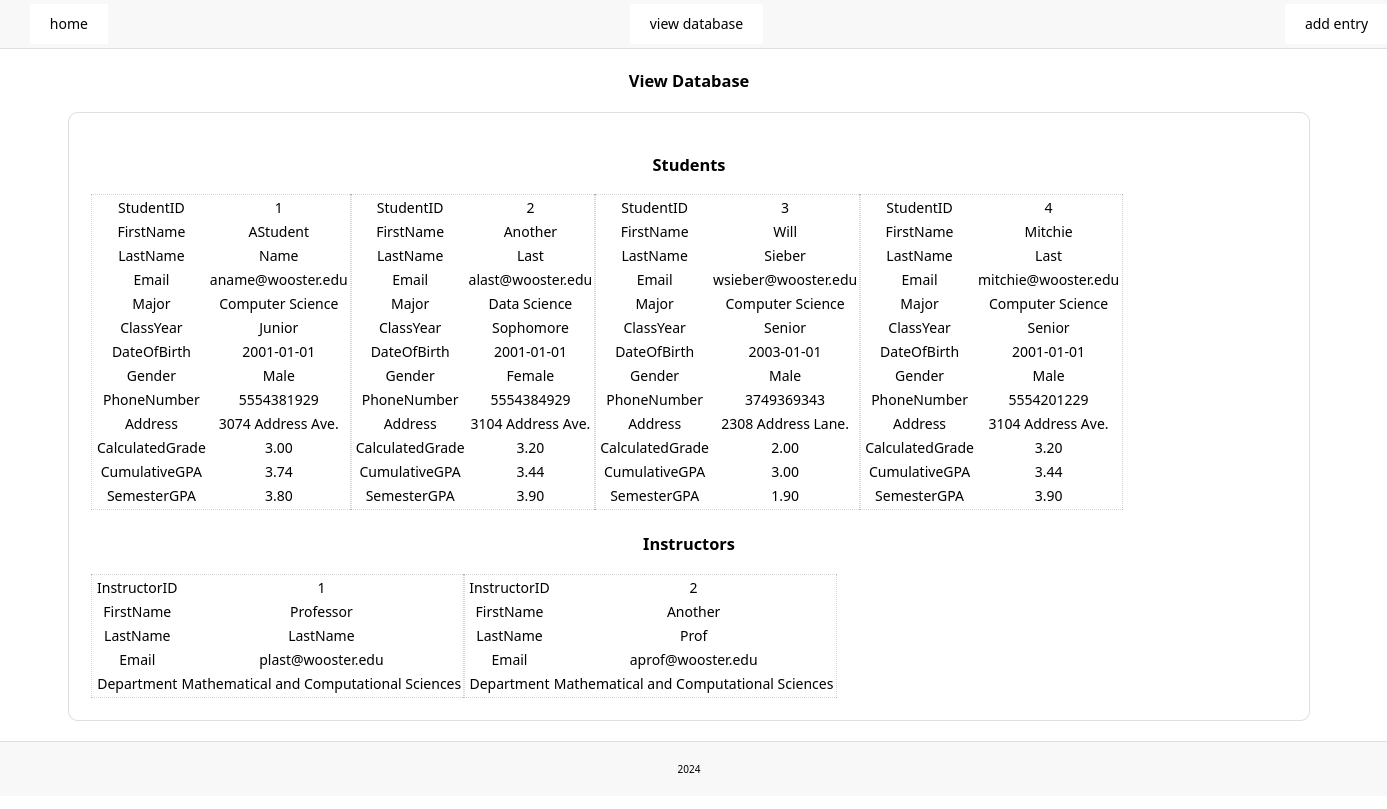
\includegraphics[width=0.8\textwidth]{images/img2.png}
    \caption{The View Database page.}
    \label{fig:mesh1}
\end{figure}


\begin{figure}[h]
    \centering
    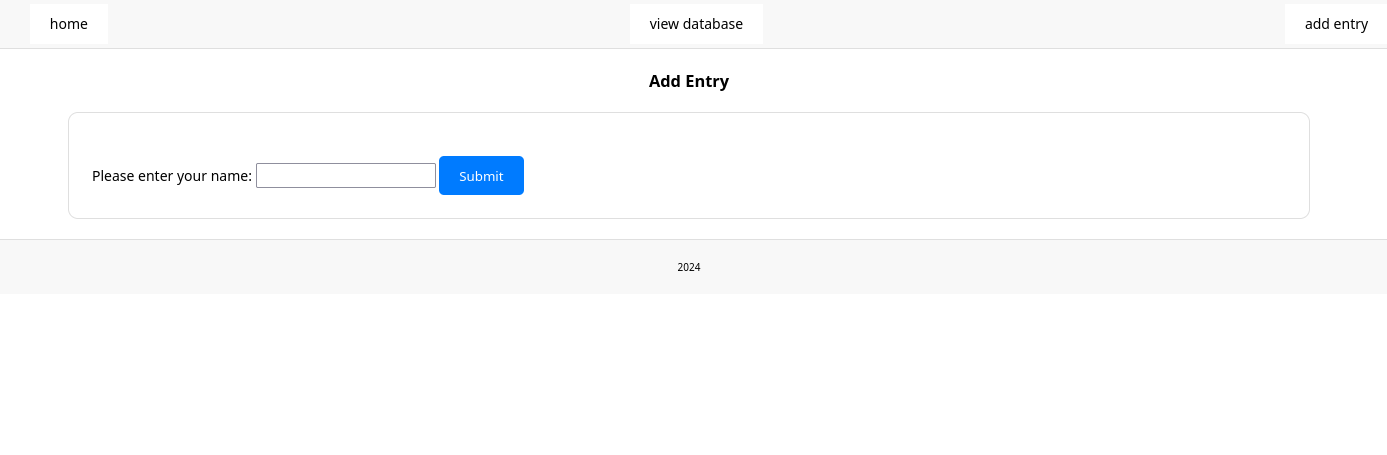
\includegraphics[width=1\textwidth]{images/img3.png}
    \caption{The Add Entry page.}
    \label{fig:mesh1}
\end{figure}

\newpage

\section{Conclusion}
\subsection{Project Overview}
Our project aimed to create an improved course scheduling system for students at The College of Wooster. We designed a database with tables for students, courses, instructors, prerequisites, enrollments, classrooms, and schedules. The database supports efficient course planning by organizing data and enabling seamless interactions, such as tracking student enrollments, course prerequisites, and classroom availability.

To ensure a user-friendly experience, we built an HTML/CSS-based interface, paired with a Golang backend for robust data handling and smooth communication between the front-end and database. The database structure allows for better insights into course selection, helping students avoid scheduling conflicts and meet prerequisites.

Throughout the project, our team communicated effectively and supported each other, ensuring smooth progress and problem-solving. Each member contributed their strengths, resulting in a well-structured, functional system. The collaborative approach and clear communication were key to the success of the project.

\subsection{Challenges and Limitations}
While functional, our database design has several limitations affecting its real-world deployment. Key issues include:

\begin{enumerate}
	\item \textbf{Grade Tracking}: Individual class grades are not tracked; only GPAs are entered at the end of each semester. This separation can lead to inconsistencies in academic records.

    \item \textbf{Front-End and Back-End Communication}: The interaction between the UI and the database needs improvement to enhance user experience and interface responsiveness.

    \item \textbf{Prerequisite Handling}: The current system does not adequately manage exceptions such as skipped prerequisites, waivers, and transferred credits, which are essential for accurate course scheduling.

	\item \textbf{Security}: Advanced security features, including data encryption, robust user authentication, and authorization protocols, are lacking and need to be strengthened.

    \item \textbf{Reporting and Analytics}: Limited reporting and analytics capabilities hinder comprehensive data analysis and decision-making processes.

    \item \textbf{Data Integrity}: Stronger data validation rules and integrity constraints are needed to maintain consistency and accuracy across the system.
\end{enumerate}


\subsection{Future Work}

The implementation of limitations on numerical fields like GPA and Credits for example would be a point of emphasis in an attempt to improve this. For credits, it would enable instructors and students to know how many credits have been attained and how many are needed to graduate in however many semesters. From here, expanding the database to include more information for students and professors can allow administrators to better manage classes on campus. For example, this can include limiting a student from taking too many credits per semester. Another addition to this expansion that could better enhance the student’s and instructor’s experience would be knowing how many credits a student needs to graduate, to help better structure their schedule if order to graduate as planned.

Nulls could mean several things and in a student database, that could lead to severe implications such as retaking a class or failing to graduate.  Limiting the number of these that can be inserted in the database would allow calculations to occur and be accurate and interpretations of the data to be more concrete and definite. From the usability perspective of things, adding a more interactive and welcoming UI to accommodate the functionality would improve the system. The addition of more buttons and sliders to give the users an alternative form of maneuvering through the database.

%\newpage
% Bibliography
%\bibliography{bibliography}
%\bibliographystyle{abbrv}

\end{document}
